\documentclass{article}
\usepackage[utf8]{inputenc}
\usepackage{listings}
\usepackage{CJKutf8}
\usepackage{amsmath}
\usepackage{graphicx}
\usepackage[export]{adjustbox}
\usepackage{tikz}
\usetikzlibrary{trees}

\title{Lab4 Report}
\author{b09901142 EE3 呂睿超}
\date{November 2022}

\usepackage{xcolor}

\definecolor{codegreen}{rgb}{0,0.6,0}
\definecolor{codegray}{rgb}{0.5,0.5,0.5}
\definecolor{codepurple}{rgb}{0.58,0,0.82}
\definecolor{backcolour}{rgb}{0.8,0.9,0.8}

\lstdefinestyle{mystyle}{
    backgroundcolor=\color{backcolour},   
    commentstyle=\color{codegreen},
    keywordstyle=\color{magenta},
    numberstyle=\tiny\color{codegray},
    stringstyle=\color{codepurple},
    basicstyle=\ttfamily\footnotesize,
    breakatwhitespace=false,         
    breaklines=true,                 
    captionpos=b,                    
    keepspaces=true,                 
    numbers=left,                    
    numbersep=5pt,                  
    showspaces=false,                
    showstringspaces=false,
    showtabs=false,                  
    tabsize=2
}

\lstset{style=mystyle}





\begin{document}
\begin{CJK*}{UTF8}{bsmi}
\maketitle

\section{Information Theory and Huffman coding}
\subsection{(a)}
\begin{table}[h!]
\centering
\begin{tabular}{l|r}
Symbol & Probability \\\hline
a & 0.2 \\
b & 0.05 \\
c & 0.005 \\
d & 0.2 \\
e & 0.3 \\
f & 0.05 \\
g & 0.045 \\
h & 0.15 
\end{tabular}
\caption{\label{tab:widgets}A table of symbols in X and their probabilities.}
\end{table}

\begin{enumerate}
\item From the definition of entropy, Entropy = $H[X] = -\sum_{j=0}^{n} p_j \log{p_j}$
Following the numerable values on the table, we can find out 

$H[X] = -(0.2\times \log{0.2}+0.05\times \log{0.05}+...+0.15\times \log{0.15}) \approx 2.53 $
\end{enumerate}
\subsection{(b)}
\begin{enumerate}
    \item The Huffman tree 
\begin{figure}[H]
    \begin{tikzpicture}[level distance=1.5cm,
  level 1/.style={sibling distance=3cm},
  level 2/.style={sibling distance=1.5cm}]
  \node {$n_{all}$}
    child {node {$n_{ad}$}
      child {node {$n_{a}$}}
      child {node {$n_{d}$}}
    }
    child {node {$n_{ehbfgc}$}
    child {node {$n_{e}$}}
      child {node {$n_{hbfgc}$}
      child{node{$n_{h}$}}
      child{node{$n_{bfgc}$}
      child{node{$n_{b}$}}
      child{node{$n_{fgc}$}child{node{$n_{f}$}}child{node{$n_{gc}$}child{node{$n_{g}$}}child{node{$n_{c}$}}}}}}
    };
\end{tikzpicture}
\end{figure}


\item The Huffman dictionary: Following the Huffman tree, we can generate the respective Huffman dictionary as following:
\begin{table}[h!]
\centering
\begin{tabular}{l|r}
Symbol & Codewords \\\hline
a & 11 \\
d & 10 \\
e & 01 \\
h & 001 \\
b & 0001 \\
f & 00001 \\
g & 000001 \\
c & 000000 
\end{tabular}
\caption{\label{tab:widgets}A table of symbols in X and their Codewords.}
\end{table}
\end{enumerate}

\subsection{(c)}
Following the Kraft Inequality, I calculated $\sum_{j=1}^{8}2^{-l(a{j})} = 2^{-2}*3 + 2^{-3} + 2^{-4} * 1 + 2^{-5}*1+2^{-6}*2 = 1$ , which verifies Kraft Inequality.

\subsection{(d)} Follow the definition, calculate the expectation of codeword length which is average length $\overline{L} = 2*(0.2+0.2+0.3)+3*0.15+4*0.05+5*0.05+6*0.05 = 2.6$
They satisfy Source Coding Theorem because $\exists \epsilon > 0 \ni \overline{L} \leq H[x] + \epsilon$

\subsection{(e)}
From the dictionary in (b), we can easily find out that the sequence {g,a,c,a,b} is encoded into {000001,11,000000,11,000001} (0000011100000011000001)

\subsection{(f)}
Following the Huffman tree, I only give the explanation of decoding the first bit. As we traverse down the tree following the bit-string 0-0-0-0-0-1..., we can find out that only when we reach the sixth bit can we find a node that represents a alphabet(g). Because all the nodes that represents a specific alphabet is a leaf node, we stop and continue to decode the next alphabet. Therefore, after decoding, the decoded string is {g,a,c,a,b}. 

\subsection{(g)}

\section{Implementation of Huffman coding}
\subsection{(a)} 
\begin{enumerate}
    \item Following the instructions, I implemented Huffman dictionary.  

    \item I used the sorting function to handle the descending order of the symbol probabilities.
    
    \item I used 2 buffers to store temporary information about the index and its total path probability.
    
    \item I used strcat function and detect parent $\neq$ 0, and traverse 'up' the created Huffman tree to create the codeword for every node.(Traverse every path from leaf to root)

    
\end{enumerate}

\subsection{(b)}
\begin{enumerate}
    \item Simply go through every alphabet in the sym-seq
    \item Find the index of the current alphabet.
    \item Use strcat function to append a new bit-string. 
    \item The encoded bit-string is 00001010000011100001. It is slightly different from the result of \emph{question 1e} because the structure of the Huffman tree in the two questions are slightly different.
\end{enumerate}

\subsection{(c)}
\begin{enumerate}
    \item I used two variables currstart and currend to maintain the current inspecting range of bit-string(which determines currstr).
    \item Using an approach similar as tree path traversing, I maintained currnode to record which node that I'm inspecting.
    \item Compair the currnode's left child and right child's representing bitstring and currstr respectively to determine the next direction to proceed. 
    \item If currnode is a leaf node(which is currnode $\leq$ 8 (which is size(dict)+1)/2)), refresh currstart to go on to the next 'single bit start'.
    \item The result is 'gacab' which is identical to the input and the result of \emph{question 1f}
\end{enumerate}


\section{The average codeword length of Huffman coding}
\subsection{(a)}
\quad In order to generate a random alphabet string with given probability, I used the method below.
\begin{enumerate}
    \item Generate a random decimal between 0 and 1. (which is seed.)
    \item Observe cumulative sum of the given prob array.
    \item Observe that the seed is in a certain area of the cumulated sum array.
    \item Find the corresponding alphabet of the area.
    \item For example, it generated 'dgehehhhhe' as the alphabet string.
    \item Using the huffman-enc implemented in \emph{question 2}
\end{enumerate}

\subsection{(b)}
\begin{enumerate}
    \item Using a array (L) to store the data length of every experiment, simply calculate the mean of L to obtain $L_{n}(R)$
    \item The histogram of the result is the figure in \emph{Appendix 2}
\end{enumerate}

\subsection{(c)}
\begin{enumerate}
    \item Using array (lr-results)to store the respective results and distribute them to their corresponding arrays(lr-10n,lr-50n,lr-100n).
    \item Use for loops to iterate through each R and n.
    \item The graph of the five curves is as the figure in \emph{Appendix 3}
\end{enumerate}
    
\subsection{(d)}
\quad Some observations of the graph are as below.
\begin{enumerate}
    \item For all three curves, as R increases, the $\overline{L}_{n}(R)$ gradually converges toward the calculated-average codeword length.
    \item Following the previous point, as n increases, its curve has less error compared to calculated-experimental codeword length horizontal line. 
    \item Almost all experiments verify the inequality that the experimental-average codeword length is larger than entropy, which is the optimal expectation of experimental codeword length.(optimality inequality) 
    \item Following the previous point, the probable reason that an experiment fail to verify the inequality is that the n and R is too small to simulate ideal experiment.
\end{enumerate}

\section{Appendix}
\subsection{the resulting Huffman dictionary}
\begin{figure}[h]
\centering
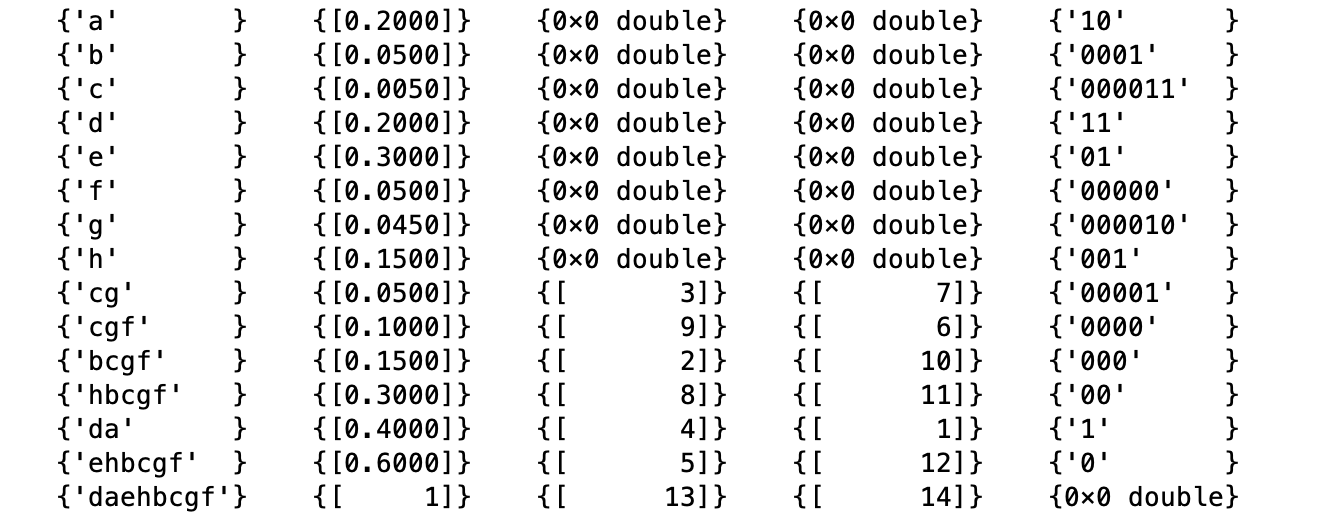
\includegraphics[width=0.7\textwidth]{huffdic.png}
\caption{\label{fig:huffdic.png}2(a) The Resulting Huffman Dictionary .}
\end{figure}

\subsection{The histogram of the result of \emph{question 3b}}
\begin{figure}[h]
\centering
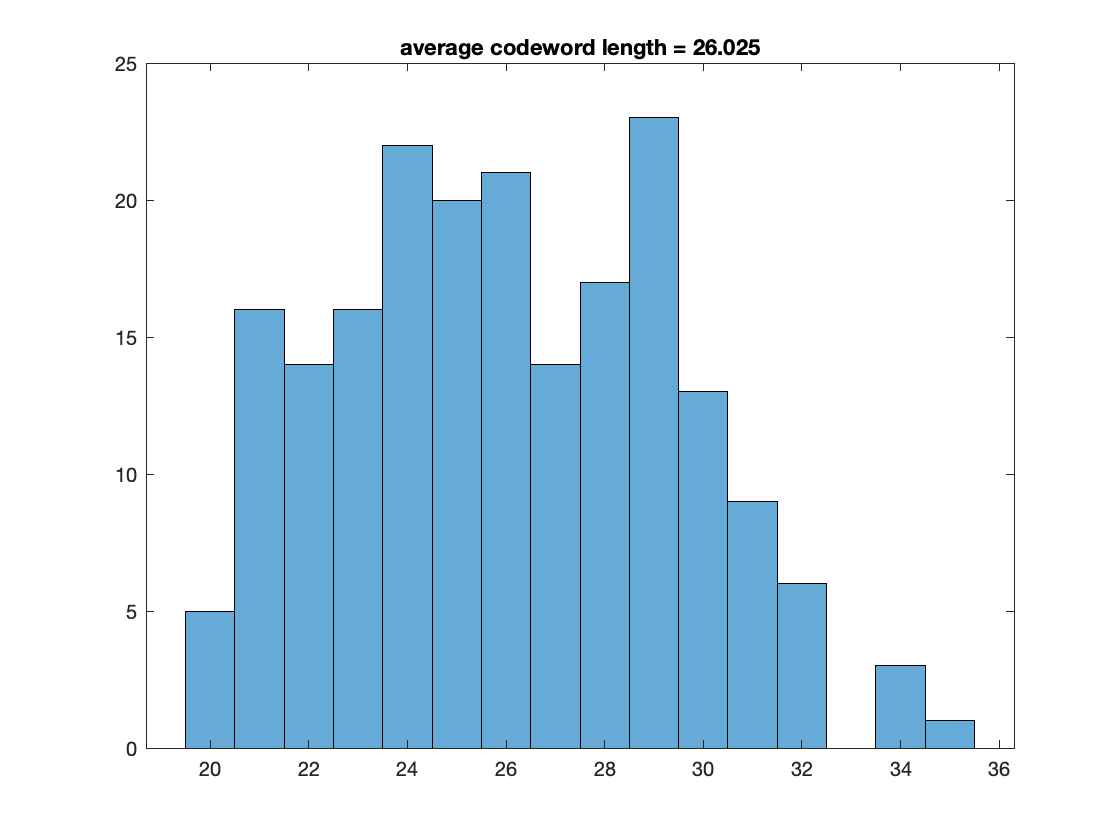
\includegraphics[width=0.8\textwidth]{3b.png}
\caption{\label{fig:3b.png}3(b) The histogram of the result of \emph{question 3b}}
\end{figure}

\subsection{The graph of the result of \emph{question 3c}}
\begin{figure}[h]
\centering
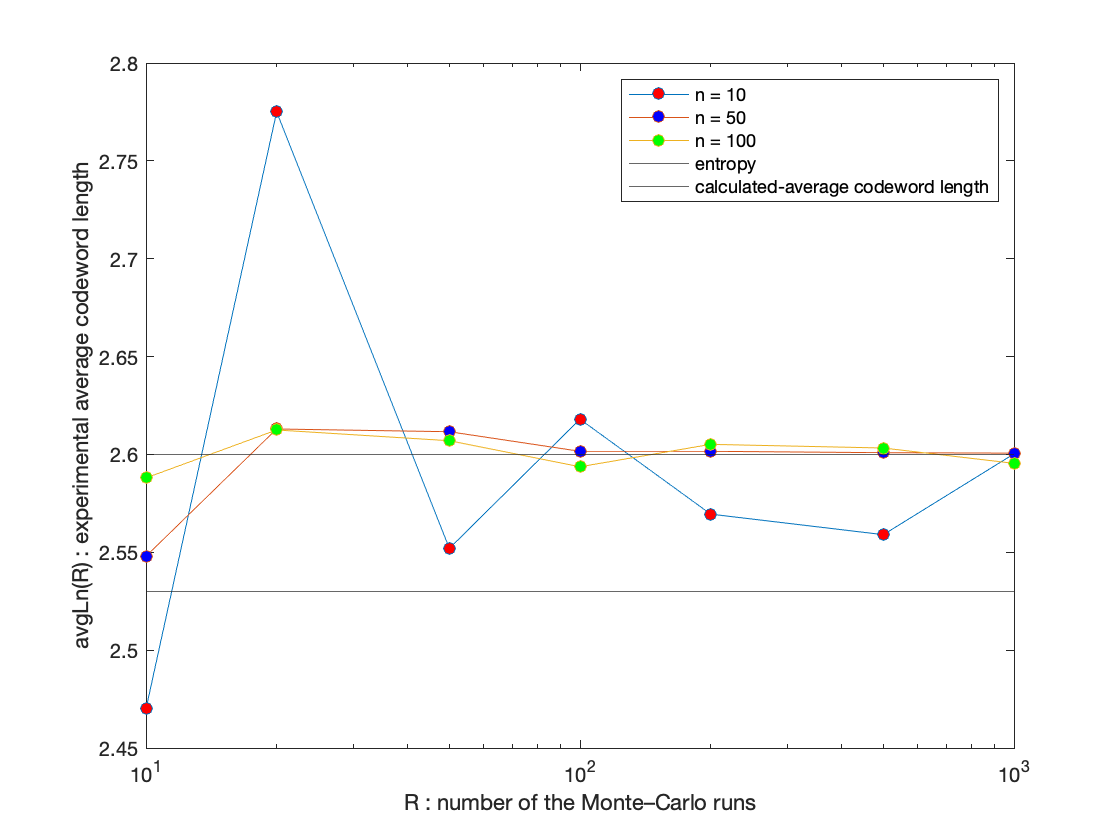
\includegraphics[width=1\textwidth]{3c.png}
\caption{\label{fig:3c.png}3(c) The graph of the result of \emph{question 3c}}
\end{figure}

\end{CJK*}
\end{document}
